\documentclass[justified]{tufte-handout}
\usepackage{../braph2_tut}
%\geometry{showframe} % display margins for debugging page layout

\title{Group of Subjects with Structural Multiplex Data}

\begin{document}

\maketitle

\begin{abstract}
\noindent
For \emph{structural multiplex data}, we will upload a file containing the structural values from different modalities (layers) for different brain areas across subjects that belong to the same group. For example, the structural values could correspond to cortical thickness or gray matter volumes obtained from T1-weighted MRI data, brain perfusion in ASL, or abnormal protein deposition in static PET data. Then a connectivity matrix is computed using correlations in structural values between each pair of brain regions for each layer, and then the layers will be integrated in a multiplex graph. This Tutorial explains how to prepare and work with this kind of data.
\end{abstract}

\tableofcontents

\fig{figure*}
	{fig:01}
	{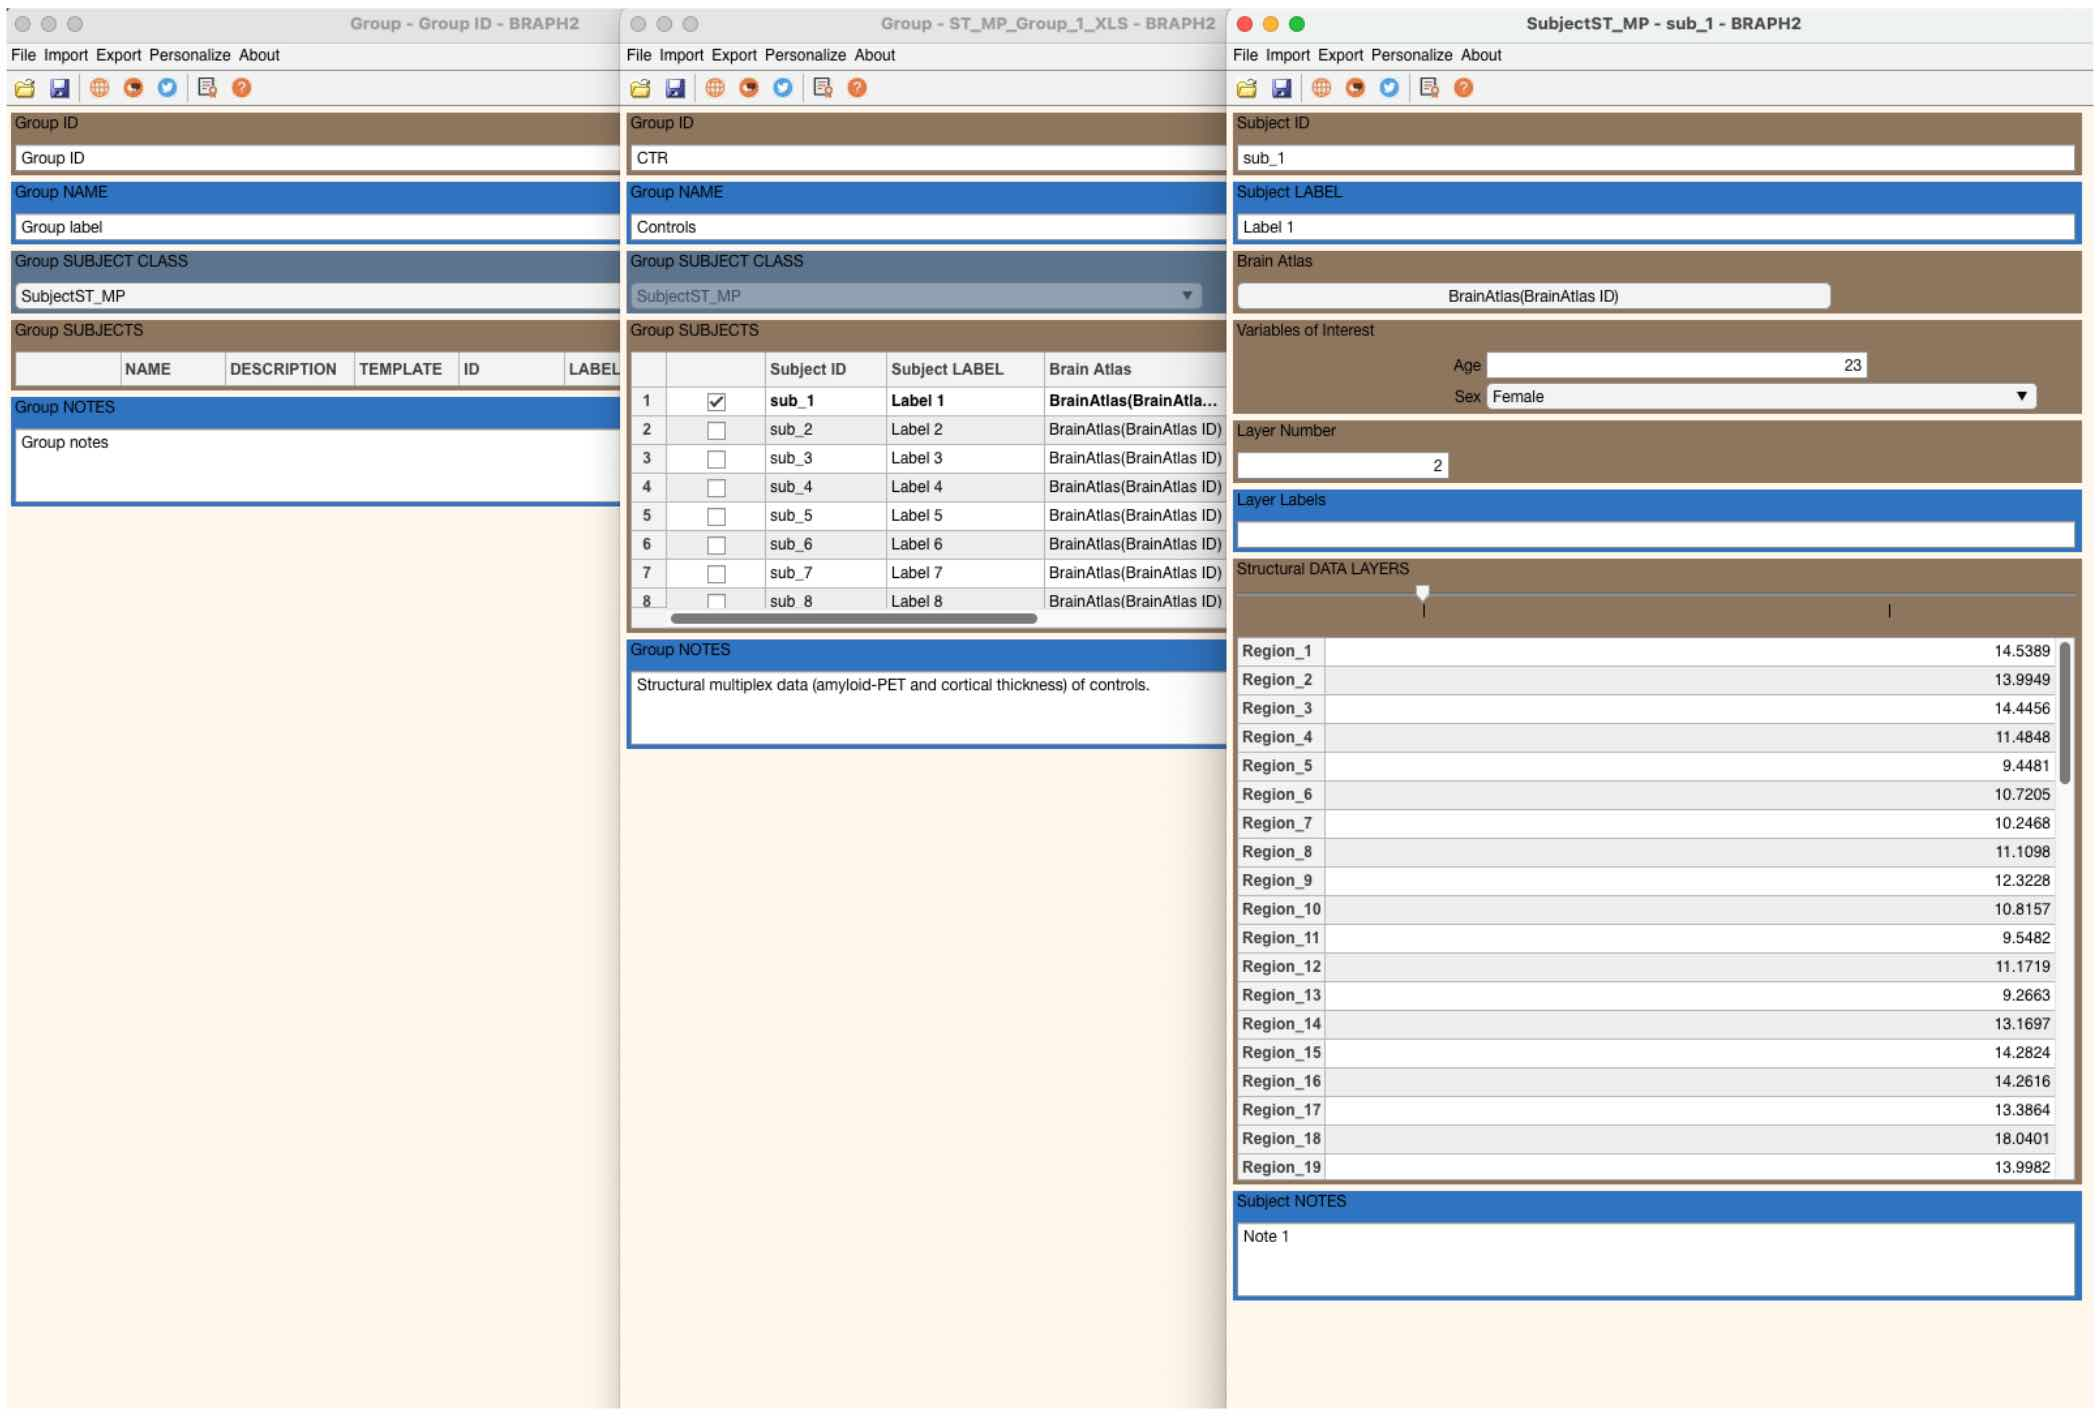
\includegraphics{fig01.jpg}}
	{GUI for a group of subjects with structural multiplex data}
	{
	Full graphical user interface to upload a group with structural multiplex data in BRAPH~2.0. 
	}

\clearpage
\section{Open the GUI}

In most analyses, the group GUI is the second step after you have selected a brain atlas. You can open it by typing \code{braph2} in MatLab's terminal, which allows you to select a pipeline containing the steps required to perform your analysis and upload a brain atlas. After these steps have been completed you can upload your group's data, as shown in \Figref{fig:02}.

\fig{figure}
	{fig:02}
	{
	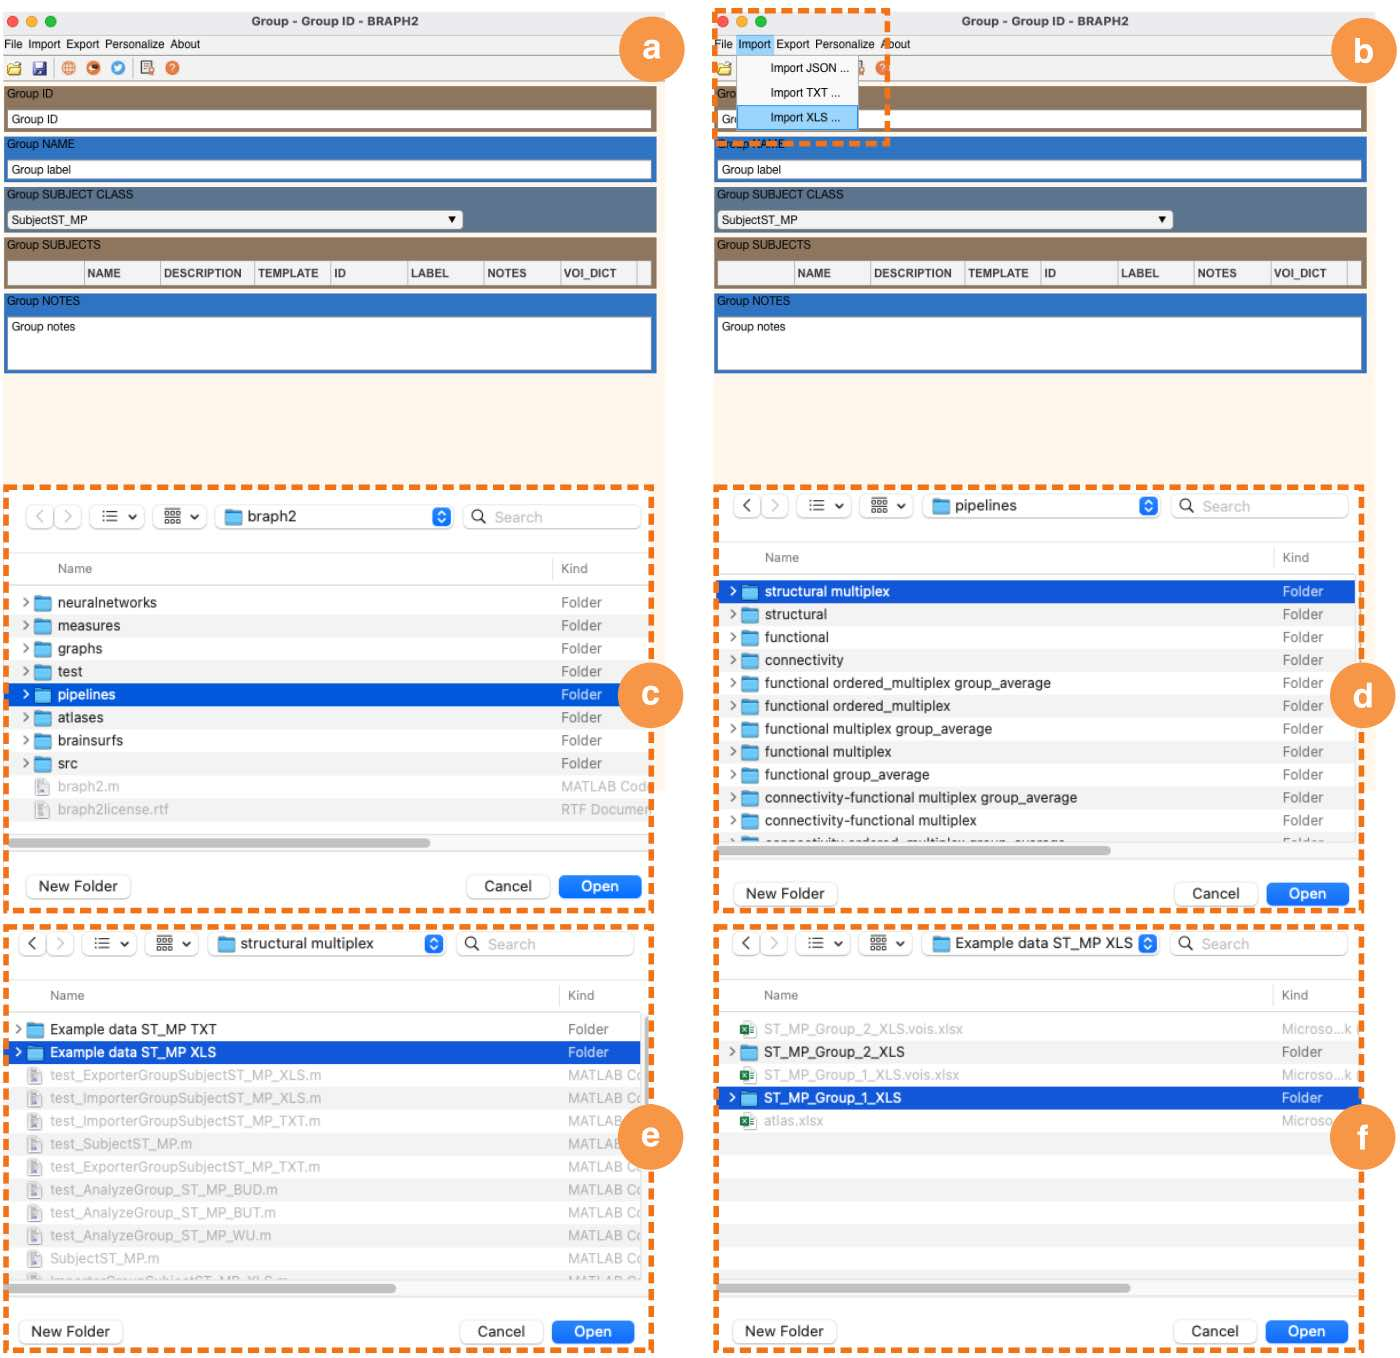
\includegraphics{fig02.jpg}
	}
	{Upload the data of a group of subjects}
	{
	Steps to upload a group of subjects with structural multiplex data using the GUI and an example dataset: 
	{\bf a} Open the group GUI.
	{\bf b} Import the folder with the structural multiplex files in XLS or TXT format (see below for details on their format).
	To upload the test structural multiplex data:
	{\bf c}-{\bf f} navigate to the BRAPH~2.0 folder \fn{pipelines}, {\bf d} \fn{structural multiplex},  {\bf e} \fn{Example data ST\_MP XLS}, and {\bf f} select the folder with structural multiplex values of one group \fn{ST\_MP\_Group\_1\_XLS}.
	}

To open the GUI and upload the brain structural multiplex data, you can also do it from the command line (i.e., without opening an analysis pipeline) by typing the commands in \Coderef{cd:launch}.
%
\begin{lstlisting}[
	label=cd:launch,
	caption={
		{\bf Code to launch the GUI to upload a group of subjects with structural multiplex data.}
		This code can be used in the MatLab command line to launch the GUI to upload a group of subjects with structural multiplex data without having to open a pipeline.
	}
]
gr = Group('SUB_CLASS', 'SubjectST_MP'); ¥\circled{1}\circlednote{1}{creates a new object \code{Group} to use structural multiplex values for assessing connectivity i.e., \code{SubjectST$\_$MP}.}¥

gui = GUIElement('PE', gr); ¥\circled{2}\circlednote{2}{creates a GUI to upload the group data.}¥
gui.get('DRAW')¥\circled{3}\circlednote{3}{draws the GUI.}¥
gui.get('SHOW') ¥\circled{4}\circlednote{4}{shows the GUI.}¥
\end{lstlisting}

Moreover, if you don't have the \fn{Example data ST\_MP XLS} folder inside \fn{structural multiplex}, then you can generate it by running the commands in \Coderef{cd:exampledata}.

\begin{lstlisting}[
	label=cd:exampledata,
	caption={
		{\bf Code to generate the example data folder.}
		This code can be used in the MatLab command line to generate the \fn{Example data ST$\_$MP XLS} folder to the \fn{structural multiplex} pipeline folder.
	}
]
test_ImporterGroupSubjectST_MP_XLS ¥\circled{1}\circlednote{1}{generates the example structural multiplex XLS data folder.}¥
test_ImporterGroupSubjectST_MP_TXT ¥\circled{2}\circlednote{2}{generates the example structural multiplex TXT data folder.}¥
\end{lstlisting}


\section{Visualize the Group Data}

After completing the steps described in \Figref{fig:02}, you can see the data (\Figref{fig:03}a), and change the Group ID, name, and notes (\Figref{fig:03}b). 

\fig{figure}
	{fig:03}
	{
	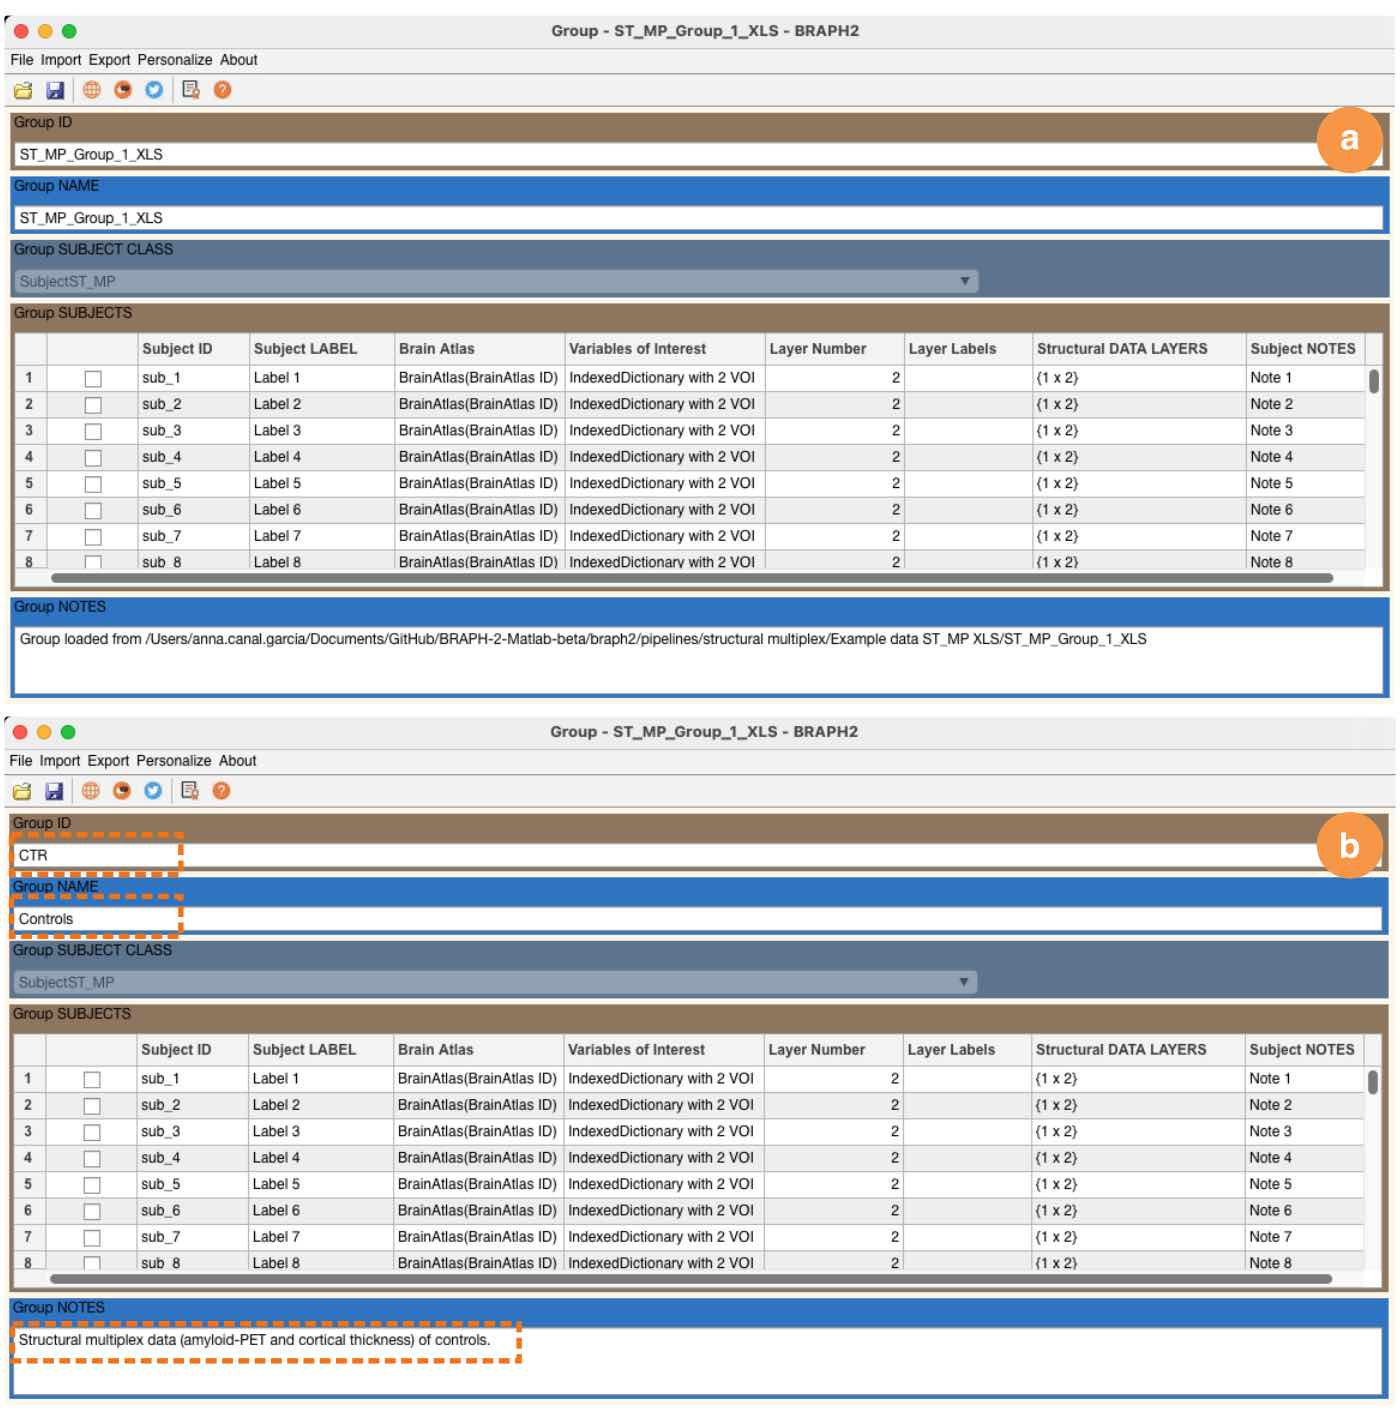
\includegraphics{fig03.jpg}
	}
	{Edit the group metadata}
	{ 
	{\bf a} The GUI of the group's structural multiplex data. 
	{\bf b} The information you see on this GUI that can be changed. In this example, we have edited the ID, name, and notes of the group but can also change the subject's specific information.
	}

\section{Visualize Each Subject's Data}

Finally, you can open each subject's structural multiplex values by selecting the subject, right click, and select ``Open selection'' (\Figref{fig:04}a), which shows the structural values from layer 1 (\Figref{fig:04}b). Here, you can also change the subject's metadata (ID, label, notes), its variables of interest, and the structural multiplex values.

\fig{figure}
	{fig:04}
	{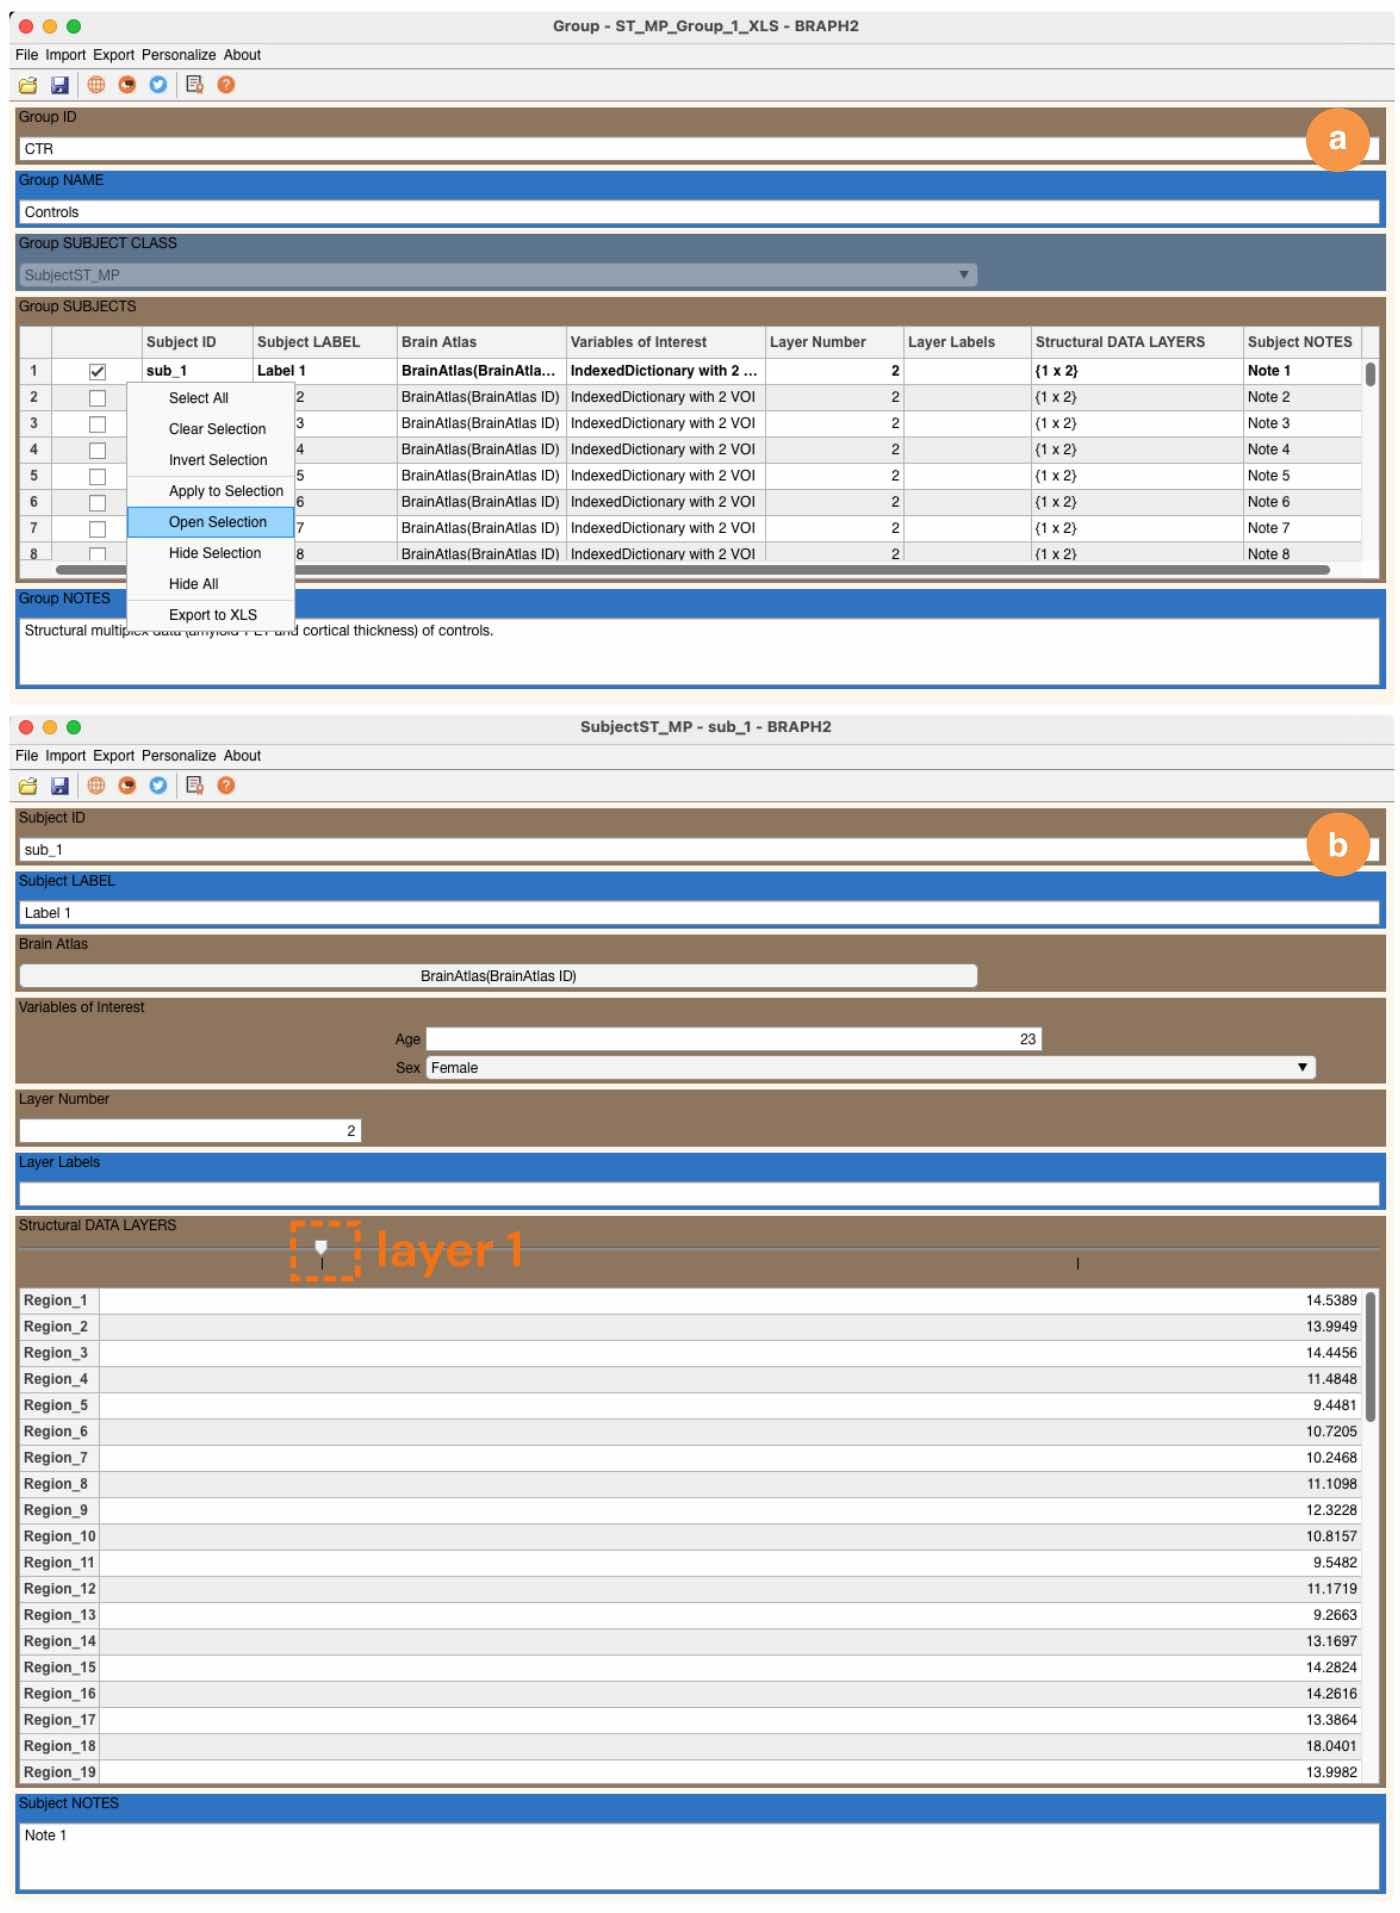
\includegraphics{fig04.jpg}
	}
	{Edit the individual subject data}
	{
	{\bf a}  Each subject's structural multiplex values can be opened by selecting the subject, right click, and select ``Open selection''.
	{\bf b} In this subject GUI, it is possible to view and edit the metadata of the subject (ID, label, notes), its variables of interest (in this case, age and sex), and the structural multiplex values. 
	}

\clearpage
\section{Preparation of the Data to be Imported}

To be able to import structural multiplex data into BRAPH~2.0, you need to include the structural values of each layer for all subjects in a single file in excel or text format. All structural layers' files should be inside one group folder. Below you can see how this file should look like.

\fig{figure*}
	{fig:05}
	{
	[h!]
	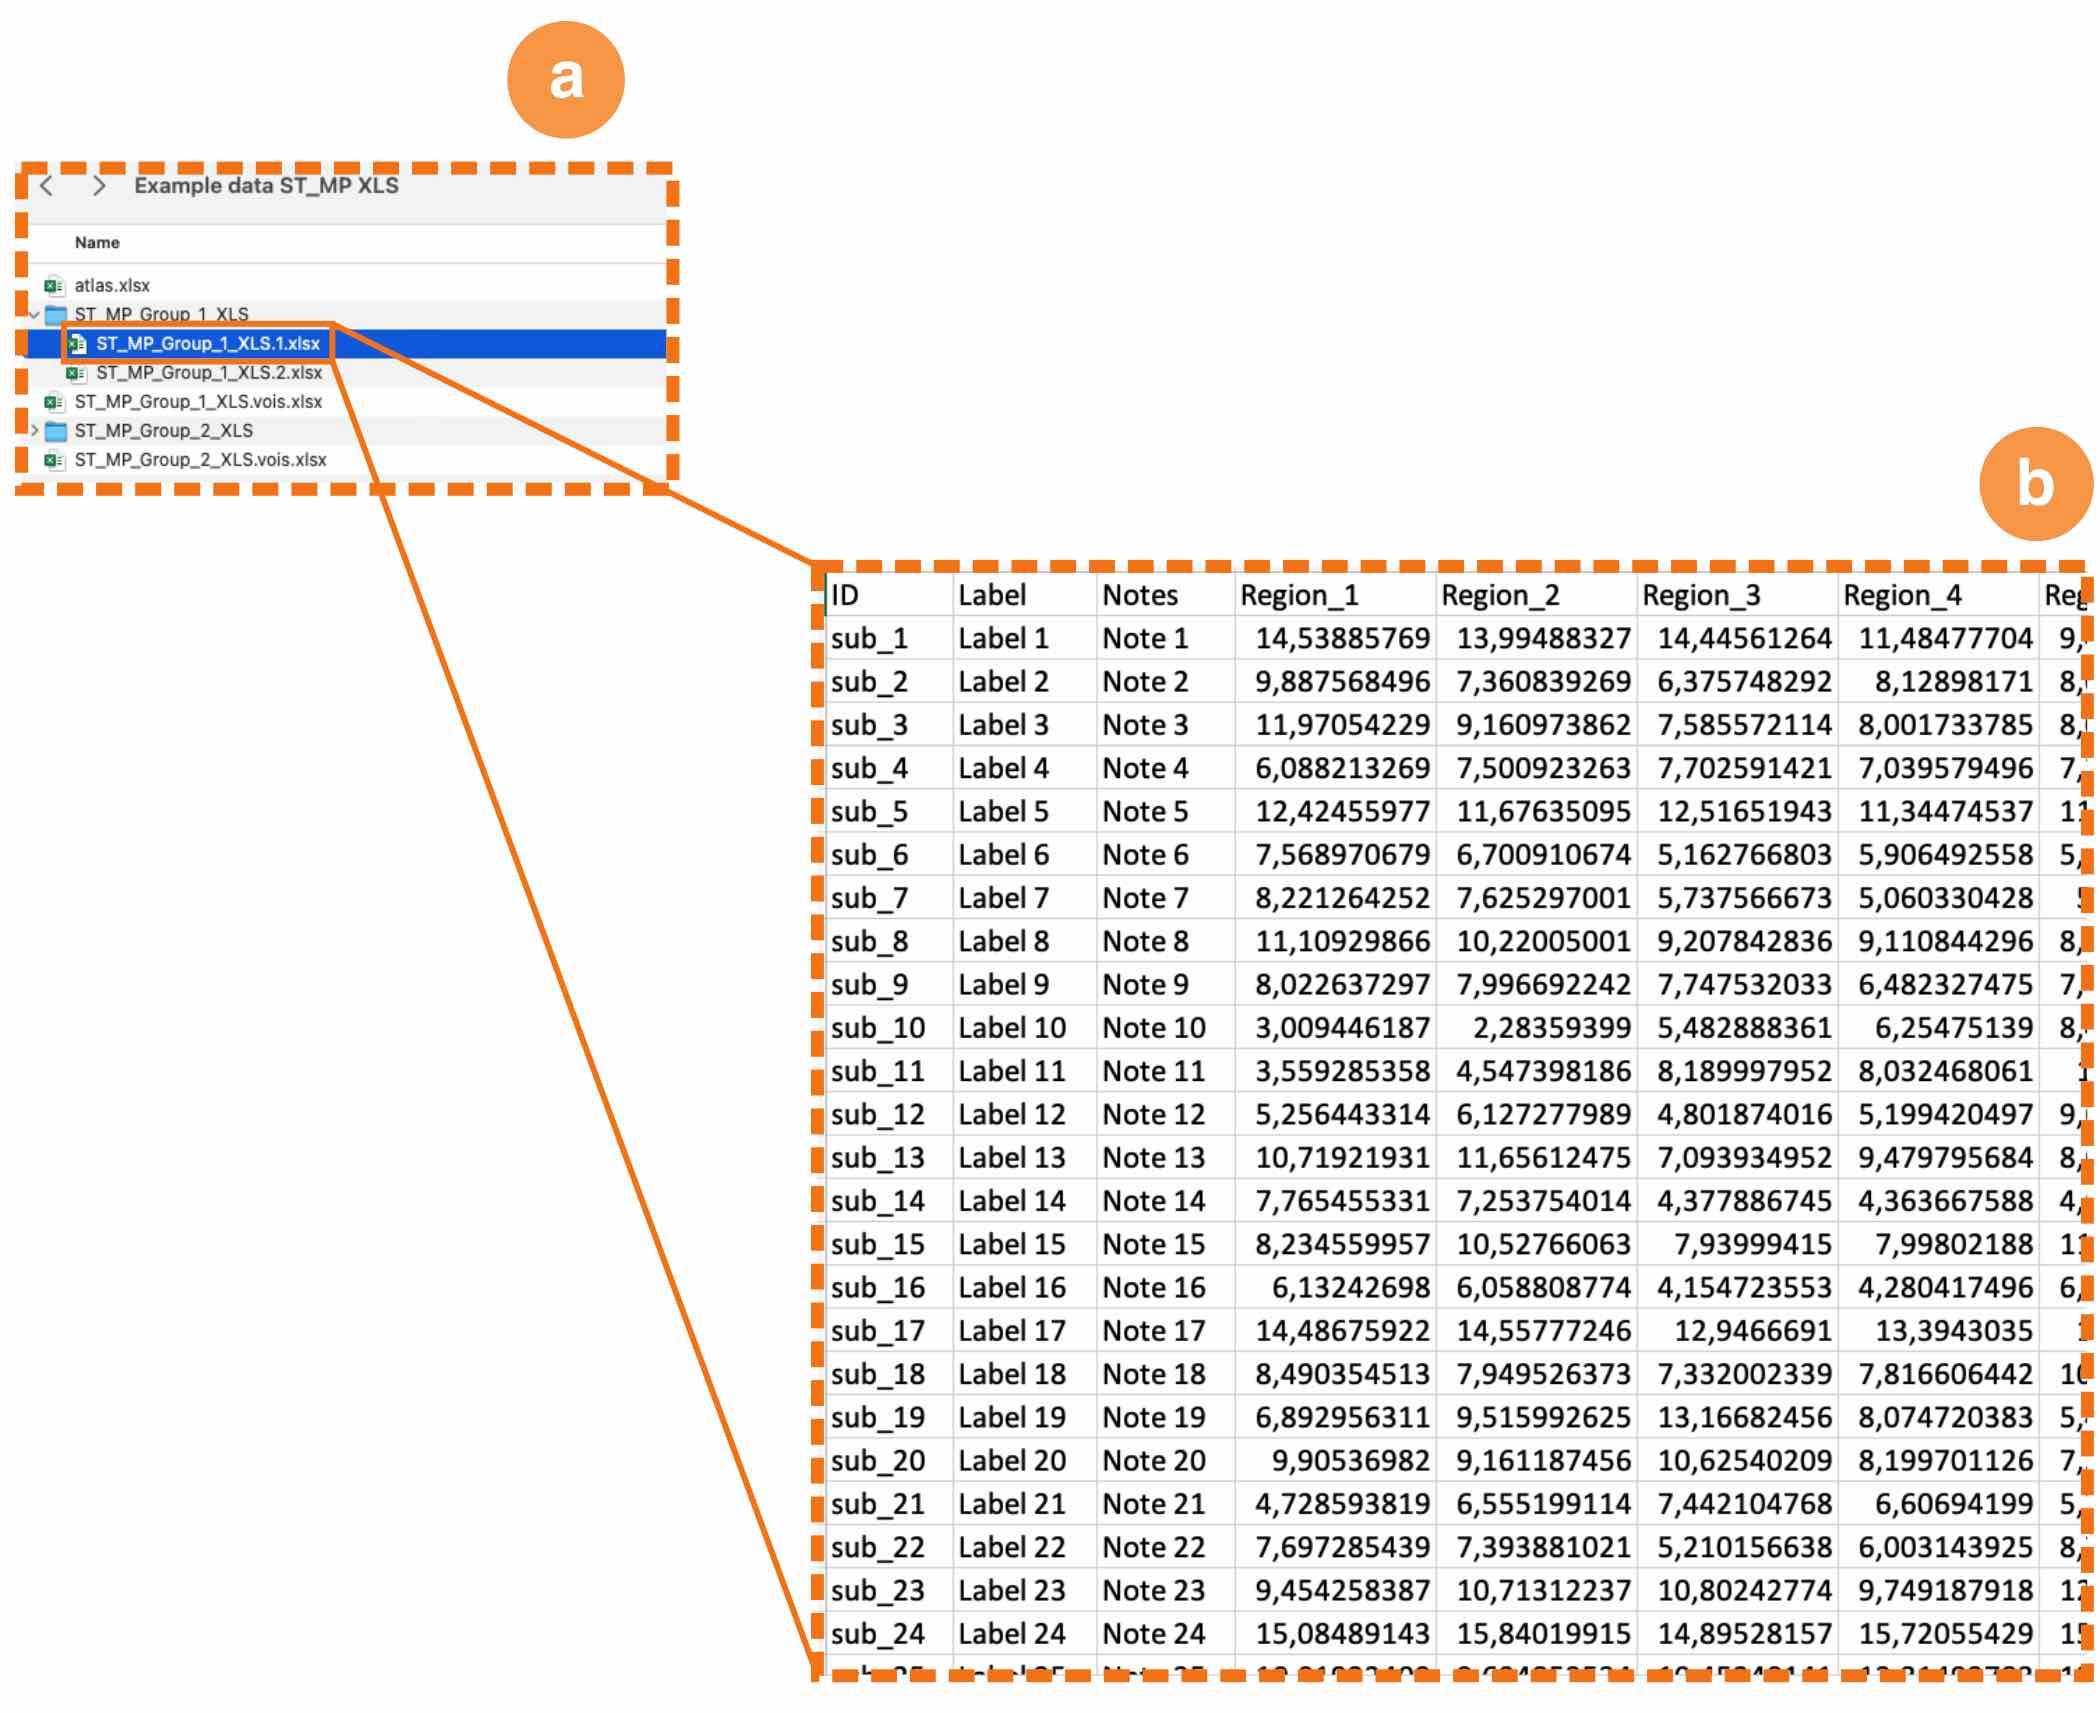
\includegraphics{fig05.jpg}
	}
	{Data preparation}
	{
	The data should be organised in the following format:
	{\bf a} The structural values of one layer from each subject belonging to the same group should be included in a single file (for example, \fn{ST\_MP\_Group\_1\_xlsx}). 
	{\bf b} This file should contain the subject's IDs, label and any relevant notes, followed by the structural values for each brain region belonging to a brain atlas. In this example, the (simulated) values correspond to the cortical thickness of 68 brain regions derived from T1-weighted MRI.
	} 

\section{Adding Covariates}

\fig{figure*}
	{fig:06}
	{
	[h!]
	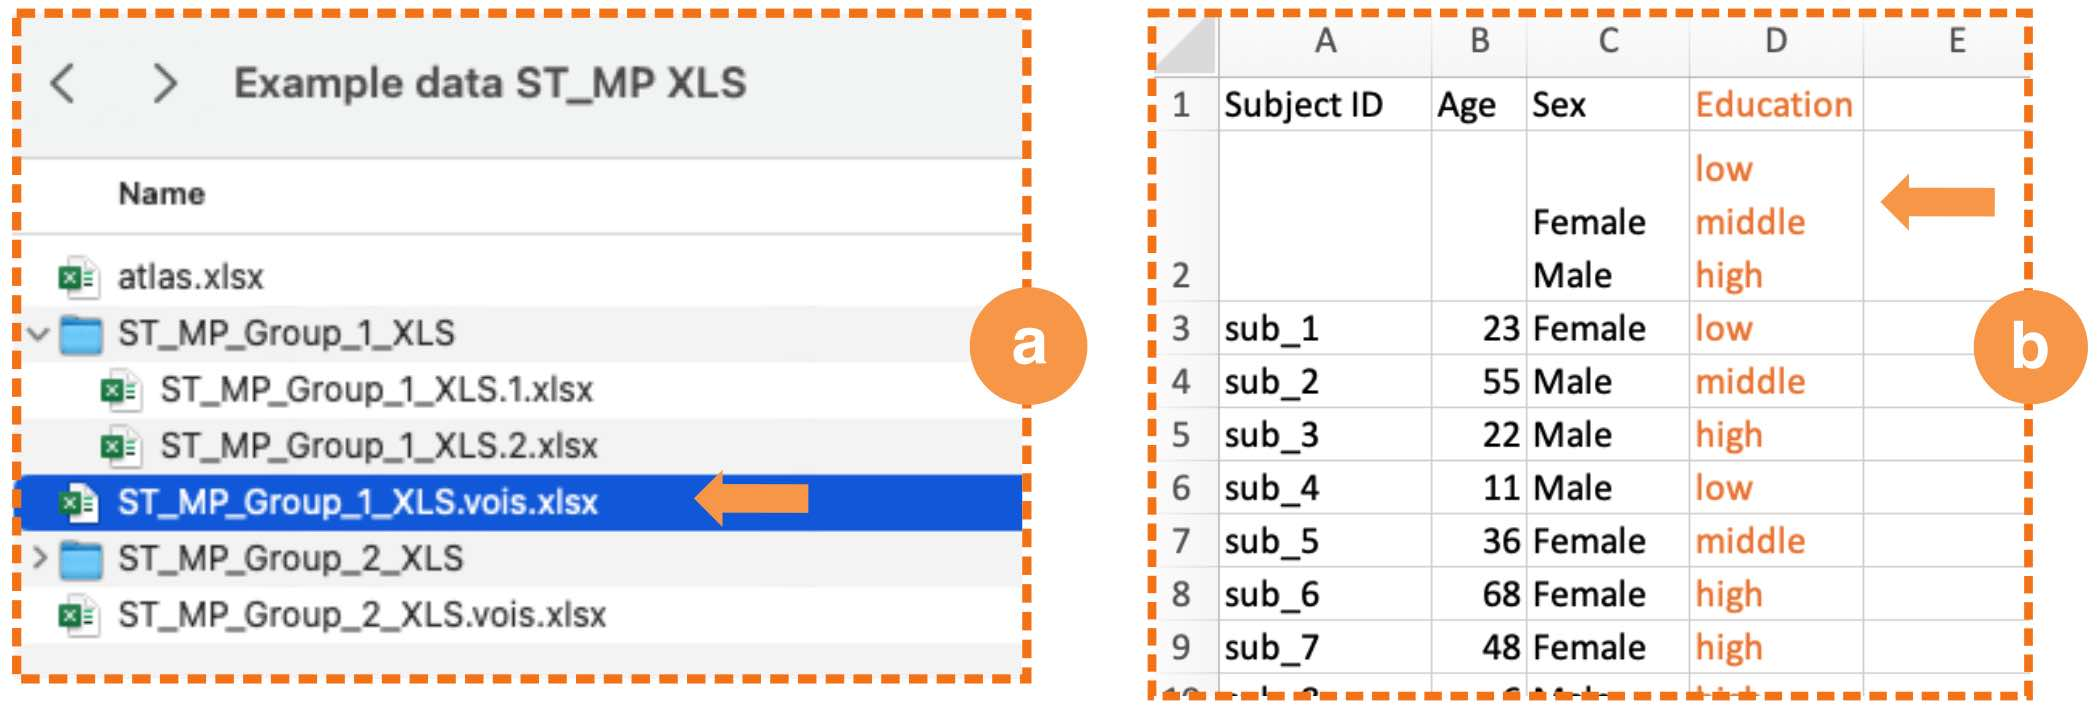
\includegraphics{fig06.jpg}
	}
	{Edit the Covariates}
	{
	Information that can be changed in the Covariates file: 
	{\bf a} The values of the variables of interest (vois).
	{\bf b} In case the vois are categorical, you can state which categories they have.
	}
	
It is very common to have \emph{variables of interest} (i.e., \emph{covariates} and \emph{correlates}) in an analysis. In BRAPH~2.0, 
these variables of interest should be included in a separate excel file placed just outside the group's folder and with the same name as the folder followed by \fn{.vois} (\Figref{fig:06}a). This file should have a specific format (\Figref{fig:06}b):
\begin{itemize}

\item[Subject IDs (column A).]
Column A should contain the subject IDs starting from row 3.

\item[Variables of interest (column B and subsequent columns).]
Column B (and subsequent columns) should contain the variables of interest (one per column). 
In this example we have ``Age'' and ``Sex'', as in the example file, as well as the additional ``Education''.
In each column, row 1 should contain the name of the variable of interest, row 2 should contain the categories separated by a return (only for categorical variables of interest, like ``Sex'' and ``Education''), and the subsequent rows the values of the variable of interest for each subject.

\end{itemize}	

\end{document}